\documentclass[11pt,a4paper]{article}
\usepackage[margin=23mm,headheight=14pt]{geometry}
\usepackage[T1]{fontenc}
\usepackage{lmodern,microtype}
\usepackage{amsmath,amssymb,bm,mathtools}
\usepackage{booktabs,tabularx,array,graphicx,float}
\usepackage[dvipsnames]{xcolor}
\usepackage{listings,enumitem}
\usepackage[font=small,labelfont=bf]{caption}
\usepackage[colorlinks=true,linkcolor=MidnightBlue,urlcolor=MidnightBlue,citecolor=MidnightBlue]{hyperref}
\usepackage{xurl}
\definecolor{curvred}{RGB}{180,24,35}
\definecolor{codebg}{RGB}{246,248,250}
\newcommand{\curv}[1]{{\color{curvred}\bm{#1}}}
\newcommand{\G}{\Gamma}
\newcommand{\gradG}{\nabla_{\!\G}}
\newcommand{\divG}{\operatorname{div}_{\G}}
\newcommand{\DG}{D_{\G}}
\newcommand{\Dt}{\mathcal D_{\G}}
\newcommand{\cv}{\mathbf c}
\newcommand{\ip}[2]{\left(#1,#2\right)_{\G}}
\newcommand{\norm}[1]{\left\lVert#1\right\rVert}
\newcommand{\R}{\mathbb R}
\newcommand{\dd}{\,\mathrm d}
\newcommand{\code}[1]{\texttt{#1}}
\newcolumntype{Y}{>{\raggedright\arraybackslash}X}
\setlength{\parindent}{0pt}
\setlength{\parskip}{5pt}
\setlength{\emergencystretch}{2em}
\setlist{nosep,leftmargin=*}
\renewcommand{\arraystretch}{1.15}
\pagestyle{plain}
\lstset{language=Python,basicstyle=\ttfamily\footnotesize,
 keywordstyle=\color{MidnightBlue}\bfseries,commentstyle=\color{OliveGreen},
 stringstyle=\color{Purple},backgroundcolor=\color{codebg},
 frame=single,rulecolor=\color{black!15},framesep=5pt,
 columns=fullflexible,keepspaces=true,showstringspaces=false,
 breaklines=true,breakatwhitespace=true,tabsize=4}
\hypersetup{pdftitle={LVPP for Eikonal equations: Taylor-Hood formulations},pdfauthor={Haojun Qin}}
\title{Surface Eikonal equations:
Taylor--Hood formulations}
\author{Haojun Qin, Brendan Keith}
\date{}

\begin{document}
\maketitle

\begin{abstract}
This note aims to correct the application of formulation (5.5) in
\cite{lvpp} to the Eikonal equation on the M\"obius strip in
Example~9, using the implementation in \cite{upstream} as a reference.
The original Taylor--Hood formulation omits an additional
curvature term arising from surface integration by parts. This omission
makes the formulation inconsistent with the Eikonal equation
whenever the curvature coupling is nonzero.
We derive the corrected weak formulation and compare the original and
corrected implementations. Numerical experiments on the M\"obius strip
exhibit a persistent error under mesh refinement for the original
formulation, providing numerical evidence that it does not converge
to the exact solution.
\end{abstract}

\vspace{-5mm}
\section{Problem setting and notation}
\label{sec:notation}

Let $\G\subset\R^3$ be a compact, connected $C^2$ surface with nonempty boundary $\partial\G$. We consider the Eikonal problem
\begin{equation}
  |\gradG u|=1\quad\hbox{in }\G\setminus\partial\G,
  \qquad u=0\quad\hbox{on }\partial\G.
  \label{eq:eikonal}
\end{equation}
The nonnegative viscosity solution is the distance function to the boundary. It is also the maximizer of
\begin{equation}
  \max_{u\in K}\int_\G u\,dS,\qquad \text{over} \;
  K=\{u\in W^{1,\infty}(\G):u|_{\partial\G}=0,
          \ |\gradG u|\leq1\ \hbox{a.e.}\}.
  \label{eq:variational}
\end{equation}

\bigskip

The following parts are about the notations.
Choose a unit normal $n$ locally and define
\begin{itemize}
    \item $P=I-n\otimes n$, which is the projection operator onto the tangent space.
    \item $\kappa=\divG n$, which is the trace of the curvature tensor.
    \item $\cv=\kappa n$, which is the the curvature vector and lies on the normal direction.
\end{itemize}

Then we also need to recall the ambient derivative and surface derivative. Consider scalar function $u$ and vector function $\tau$. 
For their extensions to a neighborhood in $\R^3$, the ambient derivatives are difined by
\begin{equation}
 \nabla\widetilde u=(\partial_j\widetilde u)_{j=1}^3,
 \quad D\widetilde\tau=(\partial_j\widetilde\tau_i)_{i,j=1}^3,
 \quad \operatorname{div}\widetilde\tau=\operatorname{tr}(D\widetilde\tau).
\end{equation}
Their surface counterparts are
\begin{equation}
 \gradG u=P\nabla\widetilde u,\qquad
 \DG\tau=(D\widetilde\tau)P,\qquad
 \divG\tau=\operatorname{tr}(\DG\tau).
 \label{eq:derivatives}
\end{equation}
These surface derivatives are independent of the extensions. In contrast,
\begin{equation}
    \nabla\widetilde u=\gradG u+(n\cdot\nabla\widetilde u)n
\end{equation} 
retains a normal derivative depending on the extension.

\section{Surface integration by parts and corrected weak form}
\label{sec:weak}
\subsection{The integration-by-parts identity}

Let $\tau:\G\to\R^3$ be an ambient vector field. Its decomposition is
\begin{equation}
  \tau=P\tau+(\tau\cdot n)n=:\tau_T+\tau_n n.
\end{equation}
By chain rule, we obtain
\[
    \divG(\tau_n n) =\gradG\tau_n\cdot n+\tau_n\divG n
    =\kappa\tau_n.
\]
Then the surface divergence depends on two parts,
\begin{equation}
\boxed{\divG\tau=\divG(P\tau)+\curv{\kappa(\tau\cdot n)}}.
 \label{eq:div-decomposition}
\end{equation}
Thus taking a surface divergence does not discard the normal component of an ambient field. Curvature couples that component into the divergence.

Apply the surface divergence theorem to the \emph{tangent} field $u\tau_T$:
\begin{equation}
 \int_\G\divG(u\tau_T)\,dS
   =\int_{\partial\G}u\tau_T\cdot\mu\,ds.
\end{equation}
And we can derive the integration-by-parts formula on the surface,
\begin{equation}
 \ip{u}{\divG\tau_T}
   =-\ip{\gradG u}{\tau}
     +\langle u,\tau\cdot\mu\rangle_{\partial\G}.
\end{equation}
Combining this with \eqref{eq:div-decomposition} yields the full identity
\begin{align}
 \ip{u}{\divG\tau}
   & = \ip{u}{\divG \tau_T} + \ip{u}{\kappa (\tau \cdot n)} \nonumber \\
   &=-\ip{\gradG u}{\tau}
    +\langle u,\tau\cdot\mu\rangle_{\partial\G}+\curv{\ip{u\cv}{\tau}}.
 \label{eq:ibp}
\end{align}
For $u|_{\partial\G}=0$, the boundary term vanishes but the curvature term remains,
\begin{equation}
 \boxed{\ip{\gradG u}{\tau}
       =-\ip{u}{\divG\tau}+\curv{\ip{u\cv}{\tau}}.}
 \label{eq:ibp-zero}
\end{equation}
The usual identity without this term holds
\begin{itemize}
    \item when $\tau$ is tangent, e.g. using Raviart--Thomas element.
    \item when the relevant curvature coupling vanishes, e.g. solving eikonal equation on the plane.
\end{itemize}

\subsection{The LVPP equations and both curvature corrections}

For a step  $\alpha_k>0$, initialization $\psi^0=0$ and using the Hellinger entropy,
the gradient form of the LVPP subproblem is \cite{lvpp}
\begin{subequations}\label{eq:primal-system}
\begin{align}
 \ip{\psi^k}{\gradG v} 
 &= \alpha_k\ip{1}{v} + \ip{\psi^{k-1}}{\gradG v},
 && \forall v\in H_0^1(\G).\label{eq:primal-a} \\
 \ip{\gradG u^k}{\tau} - \ip{\frac{\psi^k}{\sqrt{1+|\psi^k|^2}}}{\tau}
 &=0,
 &&\forall \tau\in L^2(\G;\R^3),\label{eq:primal-b}
\end{align}
\end{subequations}

Applying the surface
integration-by-parts identity to both equations gives
\begin{subequations}\label{eq:corrected-mixed}
\begin{align}
 \ip{\frac{\psi^k}{\sqrt{1+|\psi^k|^2}}}{\tau}
 +\ip{u^k}{\divG\tau}
 -\curv{\ip{u^k\cv}{\tau}}
 &=0,&& \forall \tau \in H(\text{div}) \label{eq:corrected-a}\\
 \ip{\divG(\psi^k-\psi^{k-1})}{v}
 -\curv{\ip{\cv\cdot(\psi^k-\psi^{k-1})}{v}}
 +\alpha_k\ip{1}{v}
 &=0, && \forall v \in L^2(\Gamma).\label{eq:corrected-b}
\end{align}
\end{subequations}
Here $H(\operatorname{div})$ denotes the ambient surface-divergence space
\[
 H(\operatorname{div})
 :=\left\{\tau\in L^2(\G;\R^3):
          \divG\tau\in L^2(\G)\right\},
\]
with no tangency constraint imposed on $\tau$.

At the continuous solution, the second curvature term vanishes
because $\psi^k$ and $\psi^{k-1}$ are tangent.
But weak equations using Taylor-Hood elements do not impose exact pointwise
tangency, so this term should not be dropped.

\subsection{What the uncorrected ambient system expresses}

If the first equation \eqref{eq:corrected-a} is instead
\begin{equation}
 \ip{\frac{\psi}{\sqrt{1+|\psi|^2}}}{\tau}
 +\ip{u}{\divG\tau}=0,
\end{equation}
then integration-by-parts \eqref{eq:ibp} gives
\begin{equation}
 \ip{
   \frac{\psi}{\sqrt{1+|\psi|^2}}
   -\gradG u+u\cv
 }{\tau}=0.
 \label{eq:weak-uncorrected}
\end{equation}
Consequently, the strong equation of \eqref{eq:weak-uncorrected} gives 
\begin{equation}
 \frac{\psi}{\sqrt{1+|\psi|^2}}
   =\gradG u-u\cv,
 \label{eq:uncorrected}
\end{equation}
Since $\gradG u$ is tangent and $u\cv$ lies on the normal direction, this implies
\begin{equation}
 \frac{|\psi|^2}{1+|\psi|^2}
   =|\gradG u|^2+\kappa^2u^2<1,
\end{equation}
which is a different gradient constraint.

\section{Code comparison: original and corrected formulations}
\label{sec:code}

\subsection{Original Taylor--Hood formulation after integration by parts}

The public DOLFINx implementation in \cite{upstream} uses a quadratic
ambient Lagrange vector field and a linear Lagrange scalar field.
The comparison driver \code{eikonal\_th\_curvature.py}
contains the original \code{TH} formulation and the explicitly corrected
formulation, selected by \code{TH-curvature}. Both use the same element
definitions:
\begin{lstlisting}[language=Python]
el_psi = basix.ufl.element("Lagrange", cell, 2,
                          shape=(gdim,))
el_u = basix.ufl.element("Lagrange", cell, 1)
\end{lstlisting}
On the quadrilateral surface meshes, these are continuous
$[Q_2]^3$ and $Q_1$ spaces. Neither vector space is constrained to be
tangential.

For $f=\phi=1$, the original post-integration-by-parts residual has the
following implementation, with the nonlinear expression written explicitly:
\begin{lstlisting}[language=Python]
F = (
    ufl.inner(psi / ufl.sqrt(1 + ufl.dot(psi, psi)), tau) * dx
    + u * ufl.div(tau) * dx
    + (ufl.div(psi) - ufl.div(psi_old)) * v * dx
    + self.alpha * v * dx
)
\end{lstlisting}
Here \code{psi\_old} is $\psi_h^{k-1}$, and \code{psi} and \code{u}
are $\psi_h^k$ and $u_h^k$. The two mixed couplings are the surface
divergence of the ambient test field and the surface divergence of the
latent-field increment. Their curvature contributions are not subtracted
in the original formulation.

\subsection{Corrected Taylor--Hood formulation with explicit curvature terms}

The corrected branch retains the original residual above. On each
geometric cell $K\subset\G_h$, it computes
\begin{equation}
 n_h=\text{the local unit normal},\qquad
 \kappa_h=\operatorname{div}_{\G_h}n_h,\qquad
 \cv_h=\kappa_h n_h.
 \label{eq:code-curvature}
\end{equation}
The actual additional code is
\begin{lstlisting}[language=Python]
n_h = ufl.CellNormal(mesh)
kappa_h = ufl.div(n_h)
curvature_vector = kappa_h * n_h

# F is the original divergence-form residual shown above.
if disc == "TH-curvature":
    F -= u * ufl.dot(curvature_vector, tau) * dx
    F -= v * ufl.dot(curvature_vector, psi - psi_old) * dx
\end{lstlisting}
Thus the change to the residual is precisely
\begin{equation}
\begin{aligned}
 F_{\mathrm{corrected}}-F_{\mathrm{original}}
 ={}&-\curv{(\kappa_h u_h^k,\tau_h\cdot n_h)_{\G_h}}\\
    &-\curv{(\kappa_h(\psi_h^k-\psi_h^{k-1})\cdot n_h,v_h)_{\G_h}}.
\end{aligned}
\label{eq:code-residual-difference}
\end{equation}
The first term corrects the coupling between $u_h^k$ and the divergence
of $\tau_h$. The second corrects the divergence coupling of
$\psi_h^k-\psi_h^{k-1}$ with $v_h$. Both terms are explicitly assembled
in the code and differentiated when forming the Newton Jacobian.

\begin{table}[ht]
\centering\small
\begin{tabularx}{\linewidth}{@{}lYY@{}}
\toprule
 & Original TH & Corrected TH\\
\midrule
Code option & \code{TH} & \code{TH-curvature}\\
Vector/scalar spaces & Continuous $[Q_2]^3$ / $Q_1$ & Same spaces\\
Mixed couplings & Ambient surface divergences & Same divergences, with both curvature terms\\
\bottomrule
\end{tabularx}
\caption{Direct comparison of the two formulations after integration by
parts. The corrected branch adds the two explicit terms in
\eqref{eq:code-residual-difference}.}
\label{tab:spaces}
\end{table}

\paragraph{Geometric implementation.}
The code supports degree-2 and degree-3 geometry. In both cases,
$\cv_h$ is obtained from the actual approximate surface. The coordinate element
uses the same equispaced nodes as the mesh generator. Reversing a local
normal changes the signs of both $n_h$ and $\kappa_h$, leaving $\cv_h$
and the assembled correction unchanged. Consequently a global choice
of normal is not required on the M\"obius strip.

\section{Numerical experiments}\label{sec:numerics}
\subsection{M\"obius strip, exact distance, and matched settings}
We use the parametrization
\begin{equation}\label{eq:mobius}
 X(\theta,s)=\big((2+s\cos(\theta/2))\cos\theta,
 (2+s\cos(\theta/2))\sin\theta,s\sin(\theta/2)\big),
\end{equation}
where $0\leq\theta\leq2\pi$, $-1\leq s\leq1$, and periodic condition holds
$(0,s)\sim(2\pi,-s)$. Since $X_\theta\cdot X_s=0$ and $|X_s|=1$,
the exact solution is therefore
\begin{equation}
 u^\star(X(\theta,s))=1-|s|.
\end{equation}

We compare the original formulation \code{TH} branch and
the \code{TH-curvature} branch containing both explicit corrections
in \eqref{eq:code-residual-difference}.
Their continuous $[Q_2]^3/Q_1$ solution spaces, zero initialization,
nonlinear solver, and step sizes are identical. The geometric
coordinate degree are $g=2$ or $g=3$. Each mesh has $8n\times2n$ quadrilateral
cells, with $n=2,4,8$; the center line $s=0$ is aligned with mesh edges.

The reported series uses assembly quadrature degree 16 and error
quadrature degree 20. Starting from $\alpha_1=10$, the step size
doubles, with the final step clipped to reach
$S=\sum_k\alpha_k=10^4$.

\subsection{Scalar errors and normal components}
The two errors are
\begin{equation}
 E_u=\norm{u_h-u^\star}_{L^2(\G_h)},\qquad
 E_n=\left\lVert
 \frac{\psi_h}{\sqrt{1+|\psi_h|^2}}\cdot n_h
 \right\rVert_{L^2(\G_h)}.
 \label{eq:numerical-errors}
\end{equation}
Here
\[
 u^\star(x)=
 1-\sqrt{\big(\sqrt{x_1^2+x_2^2}-2\big)^2+x_3^2}
\]
is an ambient extension of the exact distance evaluated on $\G_h$.
Here $E_u$ measures the scalar approximation error, while $E_n$
measures the deviation of
$\psi_h/\sqrt{1+|\psi_h|^2}$ from tangency to $\G_h$.

\begin{table}[H]\centering\small
\begin{tabular}{@{}rr rrrr@{}}
\toprule
 & & \multicolumn{2}{c}{Geometry degree $g=2$}
 & \multicolumn{2}{c}{Geometry degree $g=3$}\\
\cmidrule(lr){3-4}\cmidrule(l){5-6}
$n$ & DOFs & Original TH & Corrected TH & Original TH & Corrected TH\\
\midrule
2 & 944 & $5.661\!\times\!10^{-2}$ & $6.276\!\times\!10^{-4}$ & $5.653\!\times\!10^{-2}$ & $7.503\!\times\!10^{-5}$\\
4 & 3552 & $5.325\!\times\!10^{-2}$ & $7.045\!\times\!10^{-5}$ & $5.324\!\times\!10^{-2}$ & $4.690\!\times\!10^{-6}$\\
8 & 13760 & $5.148\!\times\!10^{-2}$ & $8.550\!\times\!10^{-6}$ & $5.148\!\times\!10^{-2}$ & $4.135\!\times\!10^{-7}$\\
\bottomrule
\end{tabular}
\caption{Scalar errors $E_u$. Corrected TH means the
post-integration-by-parts formulation with two explicitly assembled
curvature terms. DOFs count all mixed-space unknowns.}
\label{tab:scalar-errors}
\end{table}

\begin{table}[H]\centering\small
\begin{tabular}{@{}rr rrrr@{}}
\toprule
 & & \multicolumn{2}{c}{Geometry degree $g=2$}
 & \multicolumn{2}{c}{Geometry degree $g=3$}\\
\cmidrule(lr){3-4}\cmidrule(l){5-6}
$n$ & DOFs & Original TH & Corrected TH & Original TH & Corrected TH\\
\midrule
2 & 944 & $1.036\!\times\!10^{0}$ & $2.426\!\times\!10^{-2}$ & $1.036\!\times\!10^{0}$ & $7.289\!\times\!10^{-3}$\\
4 & 3552 & $1.020\!\times\!10^{0}$ & $6.100\!\times\!10^{-3}$ & $1.020\!\times\!10^{0}$ & $1.807\!\times\!10^{-3}$\\
8 & 13760 & $1.013\!\times\!10^{0}$ & $1.531\!\times\!10^{-3}$ & $1.013\!\times\!10^{0}$ & $4.536\!\times\!10^{-4}$\\
\bottomrule
\end{tabular}
\caption{Normal-component deviation $E_n$ for the same runs as
Table~\ref{tab:scalar-errors}. Both formulations use the same scalar
boundary treatment.}
\label{tab:normal-errors}
\end{table}

\begin{figure}[H]\centering
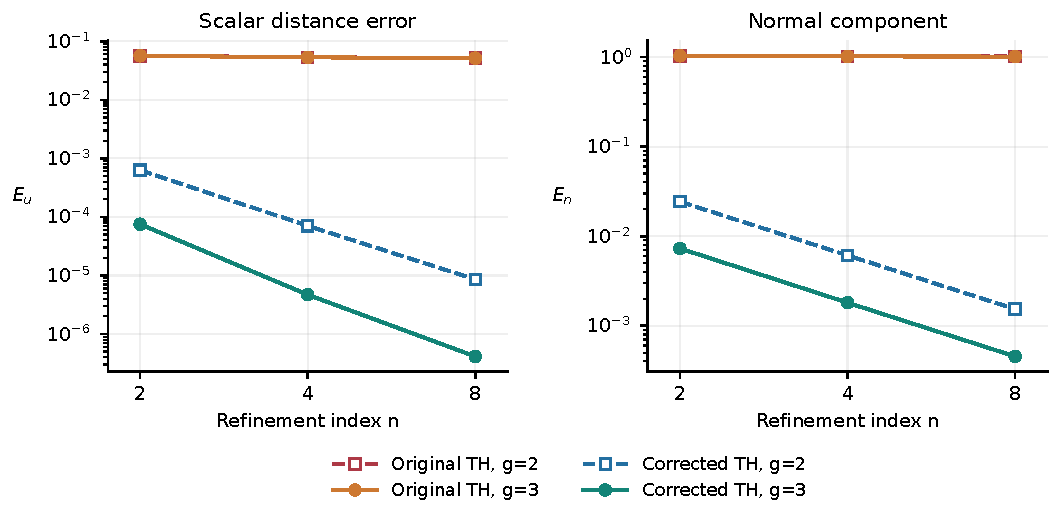
\includegraphics[width=\linewidth]{images/explicit_curvature_comparison.pdf}
\caption{Original and explicitly corrected formulation
on degree-2 and degree-3 geometric meshes.}
\label{fig:explicit-curvature}
\end{figure}

For both degree-2 and degree-3 geometry, the numerical results show
that the original TH formulation does not converge to the exact
solution under mesh refinement, whereas the TH formulation with
both explicit curvature corrections converges.

\section{Code and data reproducibility}\label{sec:reproducibility}
The driver \path{code/eikonal_th_curvature.py} implements \code{TH}
and \code{TH-curvature}; the two added terms are shown in
\path{code/curvature_terms.diff}. The reported data, source hash,
and environment record are in \path{data/explicit_curvature/quadrature16/}.
Runs used one MPI process and one BLAS/OpenMP thread with
DOLFINx 0.10.0, Basix 0.10.0, UFL 2025.2.0, and PETSc 3.24.0 with MUMPS.

From the report directory, using a compatible DOLFINx Python environment
with Matplotlib, run
\begin{lstlisting}[language=bash]
EIKONAL_PYTHON=python bash code/reproduce.sh
python make_explicit_curvature_figures.py \
    --data data/reproduced/summary.json
\end{lstlisting}
The first command reproduces all twelve cases with the settings in
Section~\ref{sec:numerics} and writes \path{data/reproduced/}.
The second regenerates \path{images/explicit_curvature_comparison.pdf}
from these results.

\begin{thebibliography}{9}\small\raggedright
\bibitem{lvpp}
J.~S. Dokken, P.~E. Farrell, B. Keith, I.~P.~A. Papadopoulos, and
T.~M. Surowiec,
\emph{The latent variable proximal point algorithm for variational problems
with inequality constraints}, Computer Methods in Applied Mechanics and
Engineering \textbf{445} (2025), 118181.
\href{https://doi.org/10.1016/j.cma.2025.118181}{doi:10.1016/j.cma.2025.118181}.
\bibitem{upstream}
METHODS Group, \emph{Proximal Galerkin}, public DOLFINx Eikonal example,
\href{https://github.com/METHODS-Group/ProximalGalerkin/blob/main/examples/09_eikonal/eikonal_dolfinx.py}{\code{examples/09\_eikonal/eikonal\_dolfinx.py}}.
\bibitem{ufl}
FEniCS Project, UFL source documentation:
\href{https://docs.fenicsproject.org/ufl/main/_modules/ufl/algorithms/change_to_reference.html}{gradient transformation to reference coordinates}
and \href{https://docs.fenicsproject.org/ufl/main/_modules/ufl/geometry.html}{Jacobian pseudoinverse on embedded meshes}.
\end{thebibliography}
\end{document}
